\documentclass[11pt,
  titlepage=false,
  abstract=on,
  %parskip=half,      % enable if you want paragraphs separated by vertical spacing instead of indents
]{scrreprt}

% Style settings
\usepackage[utf8]{inputenc}
\usepackage{microtype}
\usepackage[acronym]{glossaries}
\makeglossaries
\addtokomafont{disposition}{\rmfamily}
\renewcommand*\thesection{\arabic{section}}

% Useful packages for complex content:
\usepackage{amsmath,amsfonts,amssymb} % typesetting math
%\usepackage{siunitx}                 % typesetting SI-units and formatted numbers
\usepackage{listings}                % typesetting source code
\usepackage{booktabs,multirow}        % utils for complex/beautiful tables
%\usepackage{subcaption}              % placing multiple subfigures in a figure
\usepackage{graphicx}                % including external image files
\usepackage{tikz}                    % drawing figures within LaTeX
\usepackage{algorithm}
\usepackage{algorithmic}

% Bibliography, referencing, and indexing
\usepackage{csquotes}                 % typesetting \enquote{text in quotes} correctly
\usepackage[backend=biber,
            style=alphabetic,
            minalphanames=3, maxalphanames=4,
            maxbibnames=20]{biblatex} % to generate the bibliography
\addbibresource{report.bib}           % name of the bib-file

% Useful utils:
%\usepackage{todonotes}               % add ToDo markers (\todo{...}, \todo[inline]{...})
\usepackage[hidelinks]{hyperref}      % clickable links (but hide color frames around links)
%\usepackage{cleveref}                % named references (\Cref{sec:introduction}, ...)

% Your own macros:
%\newcommand{\mynewmacro}[1]{my content with one input parameter: #1}


\begin{document}

%--- FRONT MATTER --------------------------------------------------------------

\title{Evaluation of modular multiplication methods in lattice-based cryptography on FPGA/ASIC}
\author{Teodora-Alexandra Alexandrescu}
\date{Introduction to Scientific Working 2024/25\bigskip\bigskip}
\publishers{\normalsize
  Supervisor:
  Aikata Aikata
  \medskip\par
  Institute of Applied Information Processing and Communications\\
  Graz University of Technology
}

\maketitle


\begin{abstract}\noindent
Lattice-based cryptography is the backbone for an entire class of systems offering post-quantum security.\\
Many of these cryptosystems require rigorous mathematical approaches for laying the foundation of security, especially in the case of 
post-quantum computing or fully-homomorphic encryption schemes. A well-known NP-hard problem that is fundamental for both previously mentioned algorithms
is Ring Learning with Errors, which uses polynomial arithmetic. In several cases, if these polynomials are small and a naive computational method is used,
the performance costs will also be minimal. However, the higher the polynomial degree, the higher the need for optimization becomes.\\
To solve this problem, the concept of modular multiplication has been applied, where each coefficient in the polynomial result needs to be reduced modulo a quotient $q$ in order to reduce the coefficients. Thus, modular multiplication is the most fundamental resource in cryptographic schemes. This arithmetic operation, 
if performed efficiently, can bring a significant impact over the performance of lattice-based cryptographic implementations.\\
In this work, we address the problem of efficiency in terms of area and power consumption on digital platforms such as FPGA/ASIC
and analyze three well-known modular multipliers for evaluation: Montgomery Reduction, Barret's Reduction and Shift \& Add. Furthermore, we seek to distinguish between two novel usecases of lattice-based cryptography,
namely Post-Quantum Cryptography and Fully-Homomorphic Encryption, based on how they utilize the NP-Hard Ring Learning with Errors problem.

% Provide an abstract of your report (at most $\frac{1}{2}$ page for this report, typically 1 to 3 paragraphs).

% The abstract usually consists of two main parts: a motivational background and your contribution.
% Start with a few sentences of general introduction and background information to motivate your main research question/challenge.
% Then, summarize what your paper contributes and describe its (potential) impact.
% This includes a very short summary of all your important results and core performance numbers that characterize your approach/attack/countermeasure/implementation.
% Finally, summarize any key conclusions and calls to action that you have, e.g., apply the idea more broadly, get rid of some technology, find a countermeasure, or similar.


\paragraph*{Keywords:}
Lattice-based Cryptography $\cdot$
Post-Quantum Cryptography$\cdot$
Fully-Homomorphic Encryption$\cdot$
Modular Multipliers $\cdot$
FPGA $\cdot$
ASIC
\end{abstract}

\clearpage


%--- INTRODUCTION --------------------------------------------------------------

\section{Introduction}
\label{sec:introduction}
% To further explore the intricacies of these cryptographic schemes, 
% In asymmetric cryptography, ensuring that the private key remains secret under any circumstances is crucial. (\texttt{not entirely sure about this, 
% there's no punchline and it doesn't catch the attention of the reader. for sure an actual scientific question must be stated.})

Lattice-based constructions have gained a lot of attention in recent times due to their complexity, a characteristic that correlates with enhanced security.
As the need for secure and lightweight lattice-based algorithms increases, their complexity is also an aspect that requires intensive study, especially
in the context of platforms like FPGA or ASIC, where area and power are limited resources. Cryptosystems based on lattices derive their hardness from the
Learning with Errors problem \cite{regev2010learning}, which is considered to be as hard as an NP-hard problem \cite{micciancio2013hardness}.

Fully-Homomorphic Encryption \& Post-Quantum Cryptography are at the forefront of cryptographic research. While FHE enables computation on encrypted data, PQC
addresses threats posed by quantum-counterparts. Both FHE and PQC schemes such as \cite{gursoy2022privacy} or CRYSTALS-DILITHIUM \cite{soni2021crystals} are 
lattice-based due to how they use the (Ring -) Learning with Errors properties: the ring structure and polynomial representation. 

At the heart of these lattice-based constructions lies polynomial multiplication, which is the basic and most computationally intensive operation in Ring Learning 
with Errors cryptosystems. One crucial aspect of polynomial multiplication in lattice-based cryptography is modular multiplication, which 
ensures that the polynomial coefficients lie within manageable bounds while still keeping the initial security properties. However, the higher the security 
degree, the more convoluted these operations become and hence resources such as occupied area or power consumption need to be preserved.

For this reason, we strive to provide an evaluation of modular multiplication methods targeted on digital platforms, in order to be aware of possible bottlenecks 
or caveats during the implementation of such schemes. In this study, we will mainly discuss the Montgomery Reduction, Barrett Reduction and possible variations of them
in the context of lattice-based schemes on FPGA/ASIC.


Montgomery Reduction \cite{montgomery1985modular} is well-known for its efficiency in modular arithmetic due to replacing classical long division with bitwise operations, and by introducing the Montgomery form,
which is a precomputation step that facilitates for a faster, non-traditional division operation.
On the other hand, Barrett's modular multiplication algorithm \cite{barrett1986implementing} is more robust to changes in modulus due to the introduction of a precomputation step which highly depends on the modulus and
its bit width. The inclusion of this step enables the algorithm to eliminate division in favor of less expensive multiplication, making it efficient.

% gonna use them to smoothly transition to the background?
% To further mitigate these potential losses, we need to firstly understand the complexity of the operations
% performed within these methods.

% Modern-day experts base their encryption algorithms on hard mathematical problems such as the Learning with Errors problem to guarantee security within a certain standard.\\
% After 2005, the Learning with Errors problem published by Oded Regev \cite{regev2010learning} became a standard for cryptographic constructions due the strict security requirements it enforces.
% A study made by Micciancio \& Peikert proves its hardness to resemble the norms of approximate lattice problems in the worst case \cite{micciancio2013hardness}.
% The problem states that a secret vector $\textbf{s}$ should be retrieved from a system of linear noisy equations, where the public vector $\textbf{a}$ is drawn uniformly at random
% and the error term $\textit{e}$ is drawn from a Gaussian distribution. While it may be possible to recover the secret $\textbf{s}$
% by performing Gaussian decomposition over the system of equations, the addition of the noise term makes it computationally infeasible to retrieve the
% secret for appropriate parameters.


% The parameters provided to Learning with Errors, either number of vectors or vector dimension, usually determine the complexity of the encryption operation \cite{micciancio2013hardness}, or more specifically, the key size. 
% Cryptographic applications often need at least  $n$ vectors of $n$ dimensions, which lead to key sizes of $n^2$ \cite{regev2010learning}. This aspect can represent a challenge as the need for a higher 
% security level increases, which makes the problem inefficient for practical cryptographic applications.
% The Ring Learning with Errors problem \cite{lyubashevsky2010ideal} was introduced by Vladimir Lyubashevsky as an optimization of the initial LWE problem.

% Lyubashevsky's solution suggests a more efficient and secure approach in implementing encryption algorithms by applying the ring structure over a finite field of moduli, onto the polynomial representation 
% of public and private keys. With that being said, using polynomial multiplication within a ring structure instead of vectors and inner products should be more lightweight from a computational point of view.
% However, if we were to plainly multiply each polynomial with another, we would end up doing modulo multiplication of all coefficients with each other. When combining this method with the large parameters passed to the RLWE
% problem, the computations become highly convoluted. From a security perspective, this is beneficial, particularly in the context of FHE and PQC, which both make use of the ring property and the polynomials in afferrent applications. 
% However, the issue lies within the actual computation in the technique. For this reason, more advanced modular multiplication methods have been introduced, such as Montgomery Reduction or Barrett Reduction.



% which we are discussing in the context of Post-Quantum Cryptography and 
% Fully-Homomorphic Encryption. Moreover, we are also discussing the Shift \& Add method in combination with modular reduction, which is the basis for other modular reduction methods.

% \texttt{(the following sentences are just placeholders for now)}


% \paragraph{Our contributions: }In this paper, we want to explore these algorithms, while aiming to create an evaluation of each and every one of them in different scenarios within lattice-based cryptographic methods.
% , which facilitates
% the usage of RLWE in complex lattice-based applications such as Quantum-Safe Cryptographic Schemes and Fully-Homomorphic Encryption.

% Lattice-based applications such as Quantum-Safe Schemes and Fully-Homomorphic Encryption make use of the polynomial representation within the ring for expressing asymmetric designs. H
% However, polynomial multiplication is still an expensive operation, especially in the context of devices with limited resources such as FPGA or ASIC. The basic encryption operations require a set of RLWE parameters which define the computational properties
% of the ring structure and determine the level of security (i.e. polynomial degree). Even though the security level can be optimized, the lowest acceptable security level still yields a large ring object, of the order of millions of bits. (add reference here)
% The ring structure not only reinforces the "hardness" of 
% the initial problem, but also allows for operations on encrypted data to be performed. Both of these features facilitate the implementation of post-quantum cryptographic
% algorithms and fully-homomorphic encryption schemes.
%  by "exploiting" the structure of the LWE samples, which results in a ring over a finite
% field of moduli. The ring structure reduces the information needed to describe each vector $\textbf{a}_i$ by deriving each one of them from $\textbf{a}_1$ - this reduces the key sizes from $n^2$ to $n$. 

% ($F_q[X] / \Phi[X]$ \texttt{maybe this belongs better in the background?})

% Provide an introduction to your work (typically 1 to 2 pages, but can also be more for your full thesis).
% For this short ISW report, focus on \textbf{Introduction + Background + Conclusion} and cover them it at least \textbf{4 pages} (excluding the titlepage/abstract and bibliography).

% The introduction is structured like a longer version of the abstract.
% You start with a paragraph or two of general background, getting more and more specific, and culminating in a clear motivation for your main research problem or thesis goal.
% This should be a convincing and well-founded story: Readers will stop reading here if they do not see the relevance of your work for them.
% If you have a central research question, state it clearly.
% If there are particular papers relevant to your work, such as central techniques you used, designs you built on or evaluated, or similar, be sure to include citations here.

% Then, provide a summary and relevant details to characterize your contribution and approach for solving the research problem.
% The introduction is generally written in present tense and active form -- everything happens now and is done by ``we'', the author(s):
% ``We provide an implementation'', ``We discuss'', ``We evaluate'', etc.
% The focus is on your final \emph{outcome} and gained insights, not on your personal journey to get there; for example, do include facts like the runtime of your implementation if it is relevant for judging its performance, but do not include how many months it took you to produce this implementation.
% Provide a concise summary of your approach and your main findings, including all details already given in the Abstract and some more details.
% This includes a clear definition of the scope of your work and your assumptions, such as your attacker model, hardware/software used, and similar.
% There should be no big (positive or negative) surprises on your results for the reader in the remaining paper, except for technical details on \emph{how} you achieved your results.
% If there is a useful central figure that helps explain and contextualize your contribution, or a summary table that compares your contribution with related work, you can add it here.
% Finish this part with a (bulleted) list of around 3 to 5 main scientific contributions, such as new ideas and techniques, applications of techniques to new application areas, novel implementation results, performance numbers, and similar.

% At some point in your thesis, you need to discuss relevant related work.
% Depending on what your work contributes, a good spot for this discussion can be in the \emph{Introduction}, in the \emph{Background} section, or in a final \emph{Discussion} section.

\paragraph{Outline.}
% The introduction ends with an outline (aka mapping), explaining how this paper is structured:
% In Section \ref{sec:background}, we introduce the relevant background on some topic.
% (\dots)
% Finally, in Section \ref{sec:conclusion}, we conclude with a discussion of our findings and directions for future work.


%--- BACKGROUND ----------------------------------------------------------------

\section{Background}
\label{sec:background}

\subsection{Notation}
We use $\mathbb{Z}_q$ to represent the set of integers modulo a quotient $q \geq 2$. We represent the set of $d$-dimensional vectors in $\mathbb{Z}^d_q$
with $d \geq 1$.
\subsection{Briefly on to Lattices}
In group theory, a lattice is a discrete subgroup of the additive group, or a free abelian group of dimension $m$ which spans the vector space $\mathbb{R}^m$ and has a periodic structure. 
Each point in the lattice is separated by a minimum distance, a property that underpins the periodic nature of the lattice structure. Coordinate-wise addition or subtraction of two lattice-points 
produces a new lattice-point.

% \begin{figure}[h]
%   \centering
%   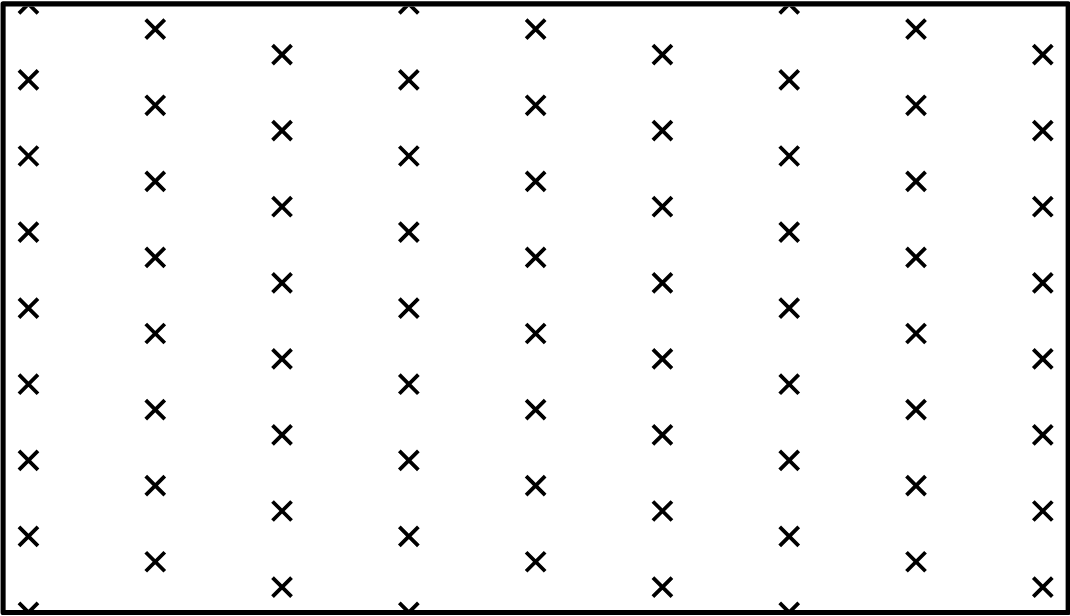
\includegraphics[width=0.6\textwidth]{figures/lattice-in-euclidean-space.png}
%   \caption{A lattice in Euclidean plane ($\mathbb{R}^2$) \cite{latticesIntro2004}}
%   \label{fig:LatticeInEuclideanPlane}
% \end{figure}



% More specifically, the lattice vectors are represented in the figure below:

\begin{figure}[h]
  \centering
  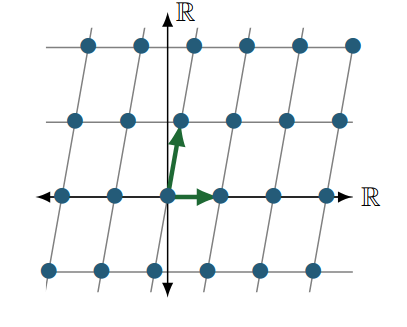
\includegraphics[width=0.6\textwidth]{figures/lattice-with-lattice-vectors.png}
  \caption{Lattice vectors in Euclidean plane \cite{latticesInPQC}}
  \label{fig:LatticeWithLatticeVectors}
\end{figure}

% \newpage

Mathematically, given $n$ linearly independent vectors $a_1, a_2,..., a_n \in \mathbb{R}^m$ as the basis, we define the lattice generated by them as follows \cite{latticesIntro2004}:
\begin{equation*}
  \Lambda(a_1, a_2,..., a_n) = \left\{\sum x_ia_i\ |\ x_i \in \mathbb{Z}\right\} 
\end{equation*}

In simpler terms, a lattice can be described as a vector space limited to integer multiples of its basis vectors.

The minimum distance of a lattice in a norm $||\cdot||$ is the length of the shortest nonzero lattice vector. If the norm is unspecified, the default
value is the Euclidean norm.

The Gaussian distribution is an important metric in lattices, especially in lattice-based cryptography where computationally infeasible problems employ the distribution
to generate random noise in order to enhance hardness. For any lattice vector $\mathbf{x}$ with a center $\mathbf{c}$ in the discreteness of the lattice, and a scaling factor $s$,
we define the discrete Gaussian distribution as follows \cite{WCToAVGCase}:

\begin{equation*}
  \rho_{s,\mathbf{c}} = e^{-\pi {\| (\mathbf{x} - \mathbf{c}) / s\|}^2}
\end{equation*}

In other words, when the discrete Gaussian distribution is applied to a lattice vector near a given center, we can generate a noisy version of the center vector, which adds controlled randomness 
to the cryptographic application.

% \cite{discreteGMeasuresLattices}
\subsection{Learning with Errors}
% We denote the Learning with Errors problem as following: $(\mathbf{a}, \langle \mathbf{a}, \mathbf{s} \rangle + e)$, where $\mathbf{a}$ is a vector
% drawn uniformly at random from $\mathbb{Z}^n_q$. The goal is to retrieve the secret vector $\mathbf{s} \in \mathbb{Z}^n_q$ given an error term
% $e$ drawn from an error.
\paragraph{Definition.} Given a lattice $\Lambda \subseteq \mathbb{R}$ with a vector basis $a_1, a_2,..., a_d$ drawn uniformly at random from $\mathbb{Z}^d_q$, a secret lattice vector $\mathbf{s}=\sum s_ia_i \in \mathbb{Z}^d_q$ 
and a noisy vector $\mathbf{e}$ drawn from a discrete Gaussian error distribution $\chi$ on $\mathbb{Z}_q$, the goal of the problem is to recover $\mathbf{s}$ from the approximated, noisy output 
$\mathbf{b} = (\mathbf{a}, \langle \mathbf{a}, \mathbf{s} \rangle + e)$. \cite{regev2010learning}\\

\[
  \begin{aligned}
  % \text{The Learning with Errors Problem:} \quad
a_1^{(1)} \cdot s_1 + \dots + a_d^{(1)} \cdot s_d &\approx b^{(1)} \pmod{q} \\
a_1^{(2)} \cdot s_1 + \dots + a_d^{(2)} \cdot s_d &\approx b^{(2)} \pmod{q} \\
&\vdots \\
a_1^{(n)} \cdot s_1 + \dots + a_d^{(n)} \cdot s_d &\approx b^{(n)} \pmod{q}
\label{The Learning with Errors Problem}
\end{aligned}
\]

\paragraph{Error distribution.}
The error distribution $\chi$ is chosen to be a normal (Gaussian) distribution. This is then rounded to the nearest integer of standard deviation ($\alpha q$, where $\alpha > 0$ is typically $\frac{1}{poly(d)}$)
and reduced modulo $q$, to ensure that the noise is small relative to the modulus.

\paragraph{Modulus.} The modulus $q$ is typically chosen to be a polynomial of the vector dimension $d$. The choice of a polynomial modulus significantly increases the size of the input, which further affects
the cryptographic application's efficiency in the favor of increasing the problem's hardness.

\paragraph{Number of equations.} Researchers have drawn the conclusion that the number of equations does not result in any changes in hardness - on the contrary, the hardness is independent of it.
This is due to a property discussed in \cite{regev2010learning}, where given a fixed polynomial number of equations,  it is possible to generate an arbitrarily large number of additional equations, 
which can be further utilized.



\subsection{Ring Learning with Errors \cite{regev2010learning}} 
Assuming that there exists some repeating "pattern'' in the LWE samples, we deduce that: if we consider $d$ to be a power of $2$, and if we assume that the $\mathbf{a}$ vectors arrive in blocks of $d$ samples
$\mathbf{a}_1, \mathbf{a}_2,..., \mathbf{a}_d \in \mathbb{Z}^d_q$, where $\mathbf{a}_1 = a_1, a_2,..., a_d$ is still chosen uniformly at random , we can conclude that the remaining vectors $\mathbf{a}_i$
can be reproduced as ($a_i,..., a_n, -a_1,..,-a_{i-1}$). This notation resembles a ring structure, where we write the rest of the $\mathbf{a}_i$ vectors in terms of $\mathbf{a}_1$, which reduces the 
complexity to $O(n)$ elements of $\mathbb{Z}_q$ as opposed to $O(n^2)$ for Learing with Errors.

Mathematically, this would imply trading the group of integers modulo $q$, $\mathbb{Z}^d_q$, for the ring of all polynomials over a finite field of moduli, $\mathbb{Z}_q / \langle x^d + 1\rangle$, which are all then reduced by $x^d + 1$
to ensure that the polynomial degree does not exceed $d-1$ (this needs to go into the notation section).
The additional requirements for this change  to take place is having the dimension $d$ be a power of two, which further guarantees that $x^d + 1$ is irreducible over the rationals in order to provide
a quotient ring structure.

With that being said, the R-LWE equivalent of the original LWE problem would be:
\begin{equation*}
  a^{(i)}(x) \cdot s(x) + e^{(i)}(x) \approx b^{(i)}(x) \pmod{x^d + 1, q}
  \label{The Ring-Learning with Errors Problem}
\end{equation*}


\paragraph{Hardness.} Solving the R-LWE problem implies a solution to the worst-case lattice problems, which are restricted to the family of $ideal\ lattices$ \cite{lyubashevsky2010ideal}. Ideal lattices are mathematical
structures that satisfy a certain symmetry condition: if ($a_1, a_2,..., a_d$) is a lattice vector, then so is the ring representation of it ($x_2,...,x_n, -x_1$).
Therefore, we can conclude that no changes over the hardness would occur in the context of Ring-Learning with Errors.
% \subsection{Polynomial multiplication}
\subsection{Modular reduction and modular multiplication}
Efficient modular multiplication and reduction are at the heart of many R-LWE cryptographic applications, which implicitly use polynomial multiplication due to the ring representation.
If we recall the R-LWE problem formula from the previous chapter
we can observe three main operations that take place:
\begin{enumerate}
  \item Polynomial multiplication between polynomials and their coefficients
  \item Modular multiplication, which involves multiplication between two terms that are then reduced by a modulus.\\
        In the case of R-LWE , the multiplication takes place between polynomials and the result is reduced by $x^n + 1$.
  \item Modular reduction, which can be easily observed in R-LWE, is done firstly to reduce the polynomial degree of the polynomial multiplication result by $x^n + 1$,
  then, the polynomial coefficients are reduced modulo $q$ to ensure they lie within a certain range.
\end{enumerate}

To streamline cryptographic schemes, it is essential that these operations are performed efficiently. One of the existing drawbacks is the modulo operation, which, 
when performed using traditional long division, is highly inefficient.


\subsection{Montgomery Reduction}
Montgomery Reduction \cite{montgomery1985modular} is an efficient method that performs modular reduction after integer multiplication ($x \cdot y\ mod\ Q$).
Its efficiency comes from replacing traditional long division with simple bitwise operations, as well as from precomputing the input values into the "Montgomery form''.
% The Montgomery form represents the input by using residue classes without affecting modular addition or subtraction. 

\paragraph{Montgomery Form.} We firstly define $Q > 1$ such that $\{x \in \mathbb{Z}\ |\ x \equiv r\ mod\ Q\}$. Then we select a radix (number base) $R = 2^n$, where 
$n = machine\ word\ size$, and $gcd(Q, R) = 1$, with $R > Q$. This choice of $R$ ensures that the computations are inexpensive by making the shifting operation possible.
If $x$ is an integer, its Q-residue conversion is:
\begin{equation*}
  xR \mod Q. 
\end{equation*}

This conversion should have no impact over addition or subtraction, because the result format in Montgomery
form is 1:1 as its integer counterpart due to the distributive law.
However, this is not the case for integer multiplication. Let $x,\ y$ be integers in the range $[0,\ Q-1]$. The Montgomery form of $x\cdot y\ mod\ Q$ is:

\begin{equation*}
  (xR\ mod\ Q)(yR\ mod\ Q)\ mod\ Q\ =\ (xyR)R\ mod\ Q.
\end{equation*}

We notice that after the multiplication, the result contains an extra $R$ that needs to be eliminated. A simple method to achieve this would be division by $R$, but
the result is not divisible by $R$ due to the modulo operation. In this case, we can employ the modular inverse of $R$, which is $R^{-1}$ with the condition that $RR^{-1} - QQ' = 1$,
and $Q'$ is the set of integers satisfying  $0 < R^{-1} < Q$ and $0 < Q' < R$.
By introducing the inverse, $R^{-1}$, the additional $R$ is reduced as follows:

\begin{equation*}
  (xR\ mod\ Q)(yR\ mod\ Q)R^{-1} \equiv (xR)(yR)R^{-1} \equiv (xyR)RR^{-1} \equiv (xy)R\ mod\ Q.
\end{equation*}
\\
Thus, we have converted the multiplication between $x, y$ in Montgomery form.

% \newpage

\paragraph{Reduction Algorithm.} 
Furthermore, we will discuss how to apply modular reduction to an integer in Montgomery form by outlining the reduction algorithm below.

\begin{algorithm}
  \caption{Montgomery Reduction (REDC)}
  \label{alg:REDC}
  \begin{algorithmic}[1]
  \REQUIRE $T, Q, R = 2^n$, where $\gcd(R, Q) = 1$.
  \renewcommand{\algorithmicensure}{\textbf{Output:}}
  \ENSURE $TR^{-1} \mod Q$
  \STATE $m \leftarrow (T \mod R)Q' \mod R$
  \STATE $t \leftarrow (T + m \cdot Q) / R$
  \IF{$t \geq Q$}
      \STATE $t \leftarrow T - Q$
  \ENDIF
  \RETURN $t$
  \end{algorithmic}
\end{algorithm}

The input $T$ is any integer, or, in our case, the product between $(x,\ y)$ in Montgomery form. $Q$ is the modulus, $R=2^n$ is the Montgomery radix or base. The condition $gcd(Q, R) = 1$
ensures that Montgomery reduction can be applied, as it requires that $R$ has a modular inverse modulo $Q$. The integer $Q'$ can be computed similarly to $R'$, 
by using the Extended Euclidean Algorithm.

The intermediate value $m$ is computed to ensure that $T+mQ$ is divisible by $R$. Knowing that $Q \cdot Q' \equiv -1\ mod\ R$,
we can infer that $Q \cdot Q' + 1$ is a multiple of $R$. By applying $Q'$ to m, we ensure that it will "undo" $Q\ mod\ R$ from the computation of $t$,
such that $(T + m \cdot Q)\ mod\ R = 0$.
To validate this, we extend $T + mQ$ as follows:

\begin{equation*}
  T + mQ \equiv T + ((T\ mod\ R)Q'\mod R)Q \equiv T + T \cdot \underbrace{QQ'}_{\text{\( QQ' \equiv -1 \mod R \)}} \equiv T-T \equiv 0 \mod R
\end{equation*}

\paragraph{Hardware implementation.} Even though the REDC algorithm delivers the desired result in an optimal manner, implementing it in hardware could lead to a 
few issues, among which the most obvious one is the computation of $N'$. In this regard, we are also presenting an iterative method that uses addition, shifts and
subtractions.

Let $R=2^n$, $gcd(R, Q)=1$, let $Q$ be odd. The multiplicands are numbers in binary representation, $x, y$, where $x = (x_{n-1}, x_{n-2},...,x_{0})_2$ and $0 \leq y \leq Q$. 
We define an accumulator value whose parity bit determines whether or not the intermediate sum needs to be adjusted by adding $Q$ or not. In both cases, we divide the result by
$2$, or we shift right by $1.$. After $n$ iterations, the attained result is $xyR^{-1} \mod Q$. \cite{montgomery1985modular}, \cite{7219961}

\begin{algorithm}
  \caption{Montgomery Reduction Hardware Implementation}
  \label{alg:montgomery}
  \begin{algorithmic}[1]
  \REQUIRE \( X, Y, Q \) and \( Q \) is odd, \( X, Y < Q \)
  \renewcommand{\algorithmicensure}{\textbf{Output:}}
  \ENSURE \( Acc \leftarrow X \times Y \times R^{-1} \mod Q \)
  \STATE \( Acc \leftarrow 0 \)
  \FOR{ \( i = 0 \) \TO \( n-1 \)}
      \STATE \( Acc \leftarrow Acc + x_i \times Y \)
      \IF{ \( r_0 = 0 \) }
          \STATE \( Acc \leftarrow Acc / 2 \)
      \ELSE
          \STATE \( Acc \leftarrow (Acc + Q) / 2 \)
      \ENDIF
  \ENDFOR
  \RETURN \( Acc \)
  \end{algorithmic}
\end{algorithm}


% For addition and subtraction, the result finds itself within the ranges $[0, 2Q-2]$, $[-Q+1, Q-1]$ respectively. If the sum exceeds $Q-1$ on the positive
% side or $0$ on the negative side, we can map the result back to $[0, Q-1]$ by either subtracting or adding $Q$.

% However, this is not the case with multiplication, where the result lies within the range $[0, Q^2 - 2Q + 1]$. To reduce the result into the range $[0, Q-1]$, we need to perform division,
% which the bottleneck in many hardware applications. By using the Montgomery form, we ensure that long division is avoided by representing the inputs as multiples of $R$.
% \newpage
\subsection{Barrett Reduction}
Barrett's reduction \cite{barrett1986implementing} started out as a technique provided by Paul Barrett in 1986 to obtain a high-speed implementation of the RSA encryption algorithm
on a digital signal processing chip. This technique achieved a two and a half second encryption time on average for $512$ bit exponent and modulus, on a first generation digital signal processor (DSP).
A digital signal processor is a multiplier accumulator (MAC) and a fast microprocessor that facilitates fast multiplication due to the multiplier unit it includes in addition to the arithmetic logic unit (ALU).

The algorithm is known for its efficiency due to replacing division by cheaper multiplication and by precomputing terms while using bitshift operations.
Required are a \textbf{fixed} modulus $M$ and a radix $R = 2^{2k}$, where $k$ is the length of the modulus. The radix and the modulus play a crucial role in the precomputation step.
In addition, the input multiplicands, $x, y$ must be elements of $[0, M-1]$.

Taking into consideration all previous input constraints, we seek to retrieve the remainder of the operation $(x \cdot y \mod M)$.
The schoolbook method presented below \cite{ModArith} first computes the quotient $q$, which is further used to compute the remainder $r$.
However, this method is not suitable for hardware implementation due to the division operation which is very expensive.
\begin{align*}
  &t = x \cdot y\\
  &q = \lfloor t / m \rfloor\\
  &r = t - q \cdot m.
\end{align*}
In this regard, Barrett's algorithm introduces the precomputation step where the floating point term $\frac{1}{m}$ is approximated by truncating it after the first $2k$ bits found after $(.)$,
and brought to a higher precision by a shift to the left by the radix $R$ which scales it. The value of the precomputed term will not change as long as the value of the modulus remains constant. \cite{4272869}
Direct division is as well avoided in the approximation step of the quotient (line 3 in the algorithm) through the division by the radix, which represents a shift to the right in hardware implementations.

\begin{algorithm}
  \caption{Barrett Reduction}
  \label{alg:montgomery}
  \begin{algorithmic}[1]
  \REQUIRE \( X, Y, M \), \( X, Y < M \)
  \renewcommand{\algorithmicensure}{\textbf{Output:}}
  \ENSURE \(X \cdot Y \mod M \)
  \STATE \( T \leftarrow X \cdot Y \)
  \STATE \( \mu \leftarrow \lfloor(1 / M) \cdot 2^{2k}\rfloor \)
  \STATE \( q \leftarrow \lfloor (T * \mu) / 2^{2k} \rfloor \)
  \STATE \( r \leftarrow T - q \cdot M \)
  \IF{ \( r \geq M \) }
      \STATE \( r \leftarrow r - M \)
  \ENDIF
  \RETURN \( r \)
  \end{algorithmic}
\end{algorithm}

\paragraph{Mathematically,} the formula for finding the remainder of $(x \cdot y \mod M)$ is given by:

\begin{align*}
  &r = T - \left\lfloor \frac{T \cdot \lfloor \frac{2^{2k}}{m}\rfloor}{2^{2k}} \right\rfloor \cdot M
\end{align*}

Which is further equal to:
\begin{align*}
  &r = T - \left\lfloor \frac{T \cdot \mu}{R} \right\rfloor \cdot M
\end{align*}

Where $T = x \cdot y$ and R is the radix.

% \newpage
\subsection{Shift \& Add}

Shift \& Add is a classic multiplication method which is mainly employed in in the context of hardware implementation.
This method is at the heart of many algorithms, ranging from cryptographic applications to graphics and image processing due to the lightweight
approach it has over the multiplication. The main idea stands in leveraging bitshift operations which are equivalent to either multiplication or division.

Therefore, given two integers $x, y$ in binary representation, the algorithm is stated as follows:

\begin{algorithm}
  \caption{Shift \& Add multiplication}
  \label{alg:montgomery}
  \begin{algorithmic}[1]
  \REQUIRE \( X, Y\ \text{in binary representation}\)
  \renewcommand{\algorithmicensure}{\textbf{Output:}}
  \ENSURE \(X \cdot Y\)
  \STATE \( Prod \leftarrow 0\ (\text{because it is computed as a sum}) \)
  \FOR{ \( i = bitlength(X) - 1 \) \TO \( 0 \)}
      \IF{ \( X[i] = 1 \) }
          \STATE \( Prod = Prod + X[i] << i \)
      \ENDIF
  \ENDFOR
  \RETURN \( Prod \)
  \end{algorithmic}
\end{algorithm}

We start from the least significant bit of either of the numbers, in our case $x$. If the current bit is $1$, we shift the value to the left by $i$ and
we add it to the $Prod$ variable. Otherwise, if the bit value is 0, nothing is done. At the end, the value of the product is returned.


% Ring Learning with Errors is at the core of many lattice-based algorithms and involves the manipulation of ring objects in polynomial form.

% Every section starts with an introductory paragraph that outlines the contents and purpose of the section:

% In this section, we provide some usage examples for bibliography and citations with \texttt{biblatex} (Section \ref{subsec:bib}) and writing tips (Section \ref{subsec:hints}).

% \subsection{Citations}
% \label{subsec:bib}

% This is an example of how to specify and cite
% a book \cite{AESbook},
% a journal article \cite{bstjShannon49},
% a conference article \cite{spKocherHFGGHHLM019},
% an informal report \cite{iacrSchneierFKR15},
% and a website \cite{webIAIK21}.
% We can also add the authors' names to the citation:
% AES is a block cipher defined by \textcite{AESbook}.

% \subsection{Writing Style}
% \label{subsec:hints}

% Writing style recommendations for English differ a bit from German:
% \begin{itemize}
%   \item Prefer short, clear sentences over long, convoluted sentences.
%   \item Prefer active voice, well-defined subjects, and meaningful verbs over passive voice, vague subjects, and vague verbs.
%   \item Do not concatenate too many nouns.
%   \item When you refer to the same thing several times consecutively, call it by the same name instead of inventing synonyms. (``Wortwiederholung'' is ok.)
% \end{itemize}
% Consider using a style checker such as Grammarly -- ask your supervisor for details.

% Rules for placing commas in English are quite easy, but also quite different from German.
% The most important ones include:
% \begin{itemize}
%   \item No comma before ``that'': ``Due to the fact that\dots''
%   \item No comma before infinitives: ``We did this to find out\dots''
%   \item No comma between subject and verb (be careful not to confuse with introductory clauses): ``Completing the list is essential.''
%   \item No comma before indispensable relative clauses: ``The function returns the key which has the highest score.''
%   \item Put a comma before and after dispensable relative clauses and other non-essential phrases: ``The key, which consists of two subkeys, is generated\dots''
%   \item Put a comma after introductory clauses: ``Consequently, we use\dots''; ``After the last step, we return\dots''; ``To complete the list, we add\dots''.
%   \item Put a comma before and after ``e.g.'' and ``i.e.'': ``A block cipher, e.g., AES.''
%     Consider using ``for example/for instance/such as'' and ``that is'' instead.
%   \item Many authors put a comma before ``and, but, for, or, nor, so, yet'' when they connect two independent clauses: ``We repeated the experiment, but the result was different.''
%     This is a matter of (your or your supervisor's) preference.
%   \item Many authors put a comma before ``and, or'' in the last element of an enumeration of three or more elements: ``Alice and Bob'', but ``Alice, Bob, and Caesar.''
%     This ``Oxford comma'' is a matter of (your or your supervisor's) preference.
% \end{itemize}

% Typesetting and other hints:
% \begin{itemize}
%   \item To typeset English `single' and ``double'' quotation marks in \LaTeX, start with \verb|`| (grave accent) and end with \verb|'| (typewriter apostrophe).
%   \item Display math formulas are introduced in the previous sentence and include punctuation (often separated by a thin space \verb|\,|): The ciphertext is computed as
%     \[C = E_K(P)\,.\]
%   \item Captions are usually above tables, but below figures, and end with a full stop.
%   \item ``This key has 128 bits'', but ``128-bit key''.
%   \item References are typically capitalized and separated by a non-breaking space \verb|~|: ``Section~\ref{subsec:bib}''.
%     Try \verb|\autoref| (\autoref{subsec:bib}) or the \verb|cleveref| package. % \Cref{sec:bib}
% \end{itemize}

% Figure \ref{fig:diagram} illustrates the data of Table \ref{tab:data}.

% \begin{figure}[htpb]
%   \centering
%   %\includegraphics[width=.5\textwidth]{figures/myimage.png}
%   \caption{Concise descriptive caption for the figure (printed below the figure).}
%   \label{fig:diagram}
% \end{figure}

% \begin{table}[b]
%   \caption{Concise descriptive caption for the table (printed above the table).}
%   \label{tab:data}
%   \centering
%   \begin{tabular}{lrr} % text columns: {l}eft-aligned, number columns: {r}ight-aligned
%     \toprule
%     Item   & \multicolumn{2}{c}{Properties} \\
%              \cmidrule{2-3}
%            & First          & Second \\
%     \midrule
%     Apple  & 5              & 100 \\
%     Pear   & 10             & 99 \\
%     \bottomrule
%   \end{tabular}
% \end{table}


%--- CONCLUSION ----------------------------------------------------------------

\section{Conclusion}
\label{sec:conclusion}

% Provide the conclusions of your short report (max. $\frac{1}{2}$ page).

% This is structured similarly to the abstract and introduction.
% However, unlike the abstract, it can be partially written in past tense (for actions you performed and results that you found) as well as future tense or conditional (for predictions what the impact of your work will be).
% Start by briefly recalling the main motivation and main goal of your work.
% Repeat the main hard facts, performance numbers, and properties of your solution/work.
% %
% Emphasize your main insights, findings, and lessons learned.
% If you do not have a dedicated discussion section, you can discuss your findings and put them into perspective.
% If you have any recommendations based on your work, phrase them here.

% Finally, you can point out open problems that call for future work, but phrased in a positive way -- as opportunities.
% There should be no complete surprises (such as significant shortcomings not discussed earlier), but you can provide some new thoughts and ideas.
% %--- ACRONYMS --------------------------------------------------------------
% \newacronym{RLWE}{RLWE}{Ring Learning with Errors}
% \newacronym{LWE}{LWE}{Learning with Errors}
% \glsaddall
% \printglossary[type=\acronymtype, title={List of abbreviations}, nonumberlist]
%--- BIBLIOGRAPHY --------------------------------------------------------------

\printbibliography[heading=subbibliography]



\end{document}
